% Created 2016-03-23 Wed 21:16
% Intended LaTeX compiler: pdflatex
\documentclass[11pt]{article}
\usepackage[utf8]{inputenc}
\usepackage[T1]{fontenc}
\usepackage{graphicx}
\usepackage{grffile}
\usepackage{longtable}
\usepackage{wrapfig}
\usepackage{rotating}
\usepackage[normalem]{ulem}
\usepackage{amsmath}
\usepackage{textcomp}
\usepackage{amssymb}
\usepackage{capt-of}
\usepackage{hyperref}
\usepackage{minted}
\usepackage[margin=0.5in]{geometry}
\author{Bachir El khadir}
\date{\textit{<2016-03-11 Fri>}}
\title{Problem set 4, ORF525}
\hypersetup{
 pdfauthor={Bachir El khadir},
 pdftitle={Problem set 4, ORF525},
 pdfkeywords={},
 pdfsubject={},
 pdfcreator={Emacs 25.1.50.1 (Org mode )}, 
 pdflang={English}}
\begin{document}

\maketitle
\begin{HTML}

\label{orgspecialblock1}

\end{HTML}


\section{Q1}
\label{sec:orgheadline1}

\textbf{1.1)}

\textbf{a)}

Some helper functions
\begin{minted}[frame=lines,linenos=true]{r}
library(png)
library(kernlab)
library(ggplot2)
library(glmnet)
source("functions.R")

crop <- function(img) crop.r(img, 160, 96)
take.grad <- function(img) grad(img, 128, 64, F)
take.hog <- function(grad.img) hog(grad.img$xgrad, grad.img$ygrad, 4, 4, 6)

plt.grad <- function(grad.img, h=128, w=64, ...) {
    plot(c(),c(), asp=1, xlim=c(0,70), ylim=c(0,130), xlab="X", ylab="Y", ...)
    for (i in 1:h){
        for (j in 1:w){
            arrows(x0=j, y0=h+1-i, x1=j+grad.img$xgrad[i,j]*5, y1=h-i+1+grad.img$ygrad[i,j]*5, length=0.01)
        }
    }
}

plt.gray <- function(img.gray, ...) image(t(img.gray)[, nrow(img.gray):1], col  = gray((0:32)/32), ...)


load.from.directory <- function(dir) {
    images = list()
    img <- sample(list.files(dir), size=1) 
    return(readPNG(file.path(dir, img)))
}
\end{minted}


Load images, convert to gray, crop if necessary, and then calculate the gradient / hod

\begin{minted}[frame=lines,linenos=true]{r}
image.pos <- load.from.directory("pngdata/pos")
image.neg.uncropped <- load.from.directory("pngdata/neg")
image.neg.gray.uncropped <- rgb2gray(image.neg.uncropped)
image.pos.gray <- rgb2gray(image.pos)
image.neg.gray <- crop(image.neg.gray.uncropped)
grad.pos <- take.grad(image.pos.gray)
grad.neg <- take.grad(image.neg.gray)
hog.pos <- take.hog(grad.pos)
hog.neg <- take.hog(grad.neg)
0
\end{minted}



And then plot
\begin{center}
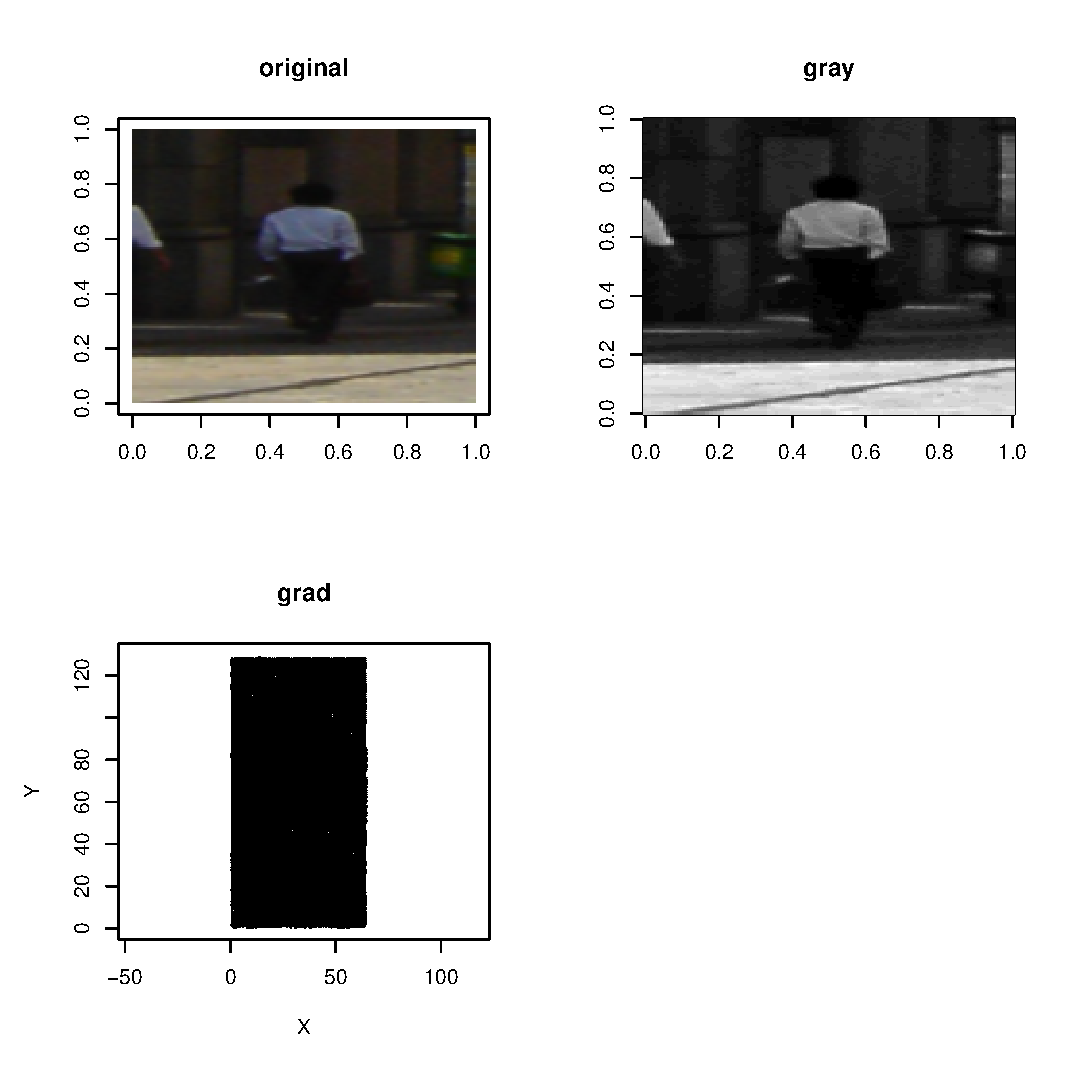
\includegraphics[width=0.75\textwidth]{./pos.eps}
\captionof{figure}{Pos image}
\end{center}

\begin{center}
\includegraphics[width=0.75\textwidth]{./neg.eps}
\captionof{figure}{Negative image}
\end{center}



\textbf{b)}

Prepare the dataset
\begin{minted}[frame=lines,linenos=true]{r}
# load all images from directory
load.all.directory <- function(dir) {
    images = list()
    for(img in list.files(dir)) {
        images[[img]] <- readPNG(file.path(dir, img))
    }
    return(images)
}

# extract features
feature.pos.img <- function(img) c(1, take.hog(take.grad(rgb2gray(img))))
feature.neg.img <- function(img) c(0, take.hog(take.grad(crop(rgb2gray(img)))))

pos.images <- load.all.directory("pngdata/pos")
neg.images <- load.all.directory("pngdata/neg")
data <- c(
    unname(lapply(pos.images, feature.pos.img)),
    unname(lapply(neg.images, feature.neg.img))
)
data <- sapply(data, identity)

# construct data frame
df <- data.frame(t(data))
colnames(df) <- c("label", paste("F",1:96, sep='_'))
df[1:3, 1:5]
\end{minted}



\textbf{1.2)}

\textbf{1)}

\(\log(C)\) take values in a uniform grid of 100 points of \([-4, 2]\). For each value, we evaluate the cross validation error of the corresponding SVM and we plot the result.
\begin{minted}[frame=lines,linenos=true]{r}
# SVM                                        
logspace <- function(s, e, n=100) 10^((1:n-1) / n * (e-s) + s)
C <- logspace(-4, 2, 10)
formula <- as.formula(paste("label", paste(colnames(df)[-1], collapse='+'), sep='~'))
cross.error <- sapply(C, function(c) {ksvm(formula, df, cross=10, C=c)@cross})
C.best <- C[which.min(cross.error)]
paste("best C", C.best)
\end{minted}

Best \(C \approx 1.58\)

\begin{org}
\begin{center}
\includegraphics[width=0.5\textwidth]{svmcrosserror.png}
\captionof{figure}{SVM cross validation error}
\end{center}
\end{org}



\textbf{2)} Now we use glmnet

\begin{minted}[frame=lines,linenos=true]{r}
x <- t(data[2:nrow(data),])
y <- data[1, ]
logit.model <- glmnet(x, y, family="binomial")
cvlogit.model <- cv.glmnet(x, y, family = "binomial", type.measure="class")
\end{minted}



\begin{org}
\begin{center}
\includegraphics[width=0.5\textwidth]{logitcrosserror.png}
\captionof{figure}{Logit error}
\end{center}
\end{org}



\textbf{3)} Compare

\begin{org}
\begin{center}
\captionof{table}{Cross validation classification error}
\begin{tabular}{rrr}
SVM & Logit 1st Lambda & Logit min Lambda\\
0.066 & 0.103 & 0.099\\
\end{tabular}
\end{center}
\end{org}

The errors are of the same order of magnitude.

\section{Q2}
\label{sec:orgheadline2}
\textbf{(a)}

\(p(x) = p(x | Y = 1) p(Y = 1) +  p(x | Y = -1) p(Y = -1) = \frac13 \frac{1_{[-5, 10]}}{15} +  \frac23 \frac{1_{[-10, 5]}}{15}\)

\[p(y | x) = \frac{ p(x | y)}{p(x)} p(y) \equiv
\left\{\begin{array}{cc}
p(Y = 1) p(x | Y=1)  & \text{if } y = 1\\
p(Y = -1) p(x | Y=-1)  & \text{if } y = -1
\end{array}\right.
\]

The bayes classifier \(B(x) := \arg \max_{y \in \{0, 1\}} p(y | x)\)
$$B(x) = 1 \iff p(Y = 1)p(x|Y=1) \ge p(Y = -1)p(x|Y=-1) \iff  1_{[-5, 10]}(x) \ge 2 \times 1_{[-10, 5]}(x) \iff x \in (5, 10)$$

\[B(x) =
\left\{\begin{array}{cc}
1 & \text{if } x \in (5, 10)\\
-1 & \text{o.w}
\end{array}
\right.
\]

Bayres Risk \(R(B) = E[1_{B(X) \ne Y}] = P(Y = 1, X \in (-5, 5)) = P(X \in (-5, 5) | Y = 1)P(Y = 1) = \frac23 \times \frac13 = \frac29\)

\textbf{(b)}

\(R(h) = E[1_{h(X) \ne Y}] = P(sign(\alpha  + \beta X^2) < 0 | Y = 1)P(Y = 1) +  P(sign(\alpha  + \beta X^2) > 0 | Y -= 1)p(Y = -1) = \frac13 \left( P_{U \sim \mathcal U([-5, 10])}(sign(\alpha  + \beta U^2) < 0) + 2 P_{U \sim \mathcal U([-10, 5])}(sign(\alpha  + \beta U^2) > 0)\right)\)

If \(\alpha\) and \(\beta\) have the same signs, then \(\alpha + \beta X^2\) keeps a constant sign.
If not, then \(\alpha + \beta X^2\) has two roots \(\pm \sqrt{\frac{-\alpha}{\beta}}\), and has the sign of \(\alpha\) only between them. Let \(r = \sqrt{\frac{-\alpha}{\beta}}\)
Cases:
\begin{itemize}
\item \(\alpha = 0, \beta = 0\) ??
\item \(\alpha \ge 0, \beta > 0\) or \(\alpha > 0, \beta \ge 0\), \(sign(\alpha + \beta X^2)  = 1\), \(R(h) = \frac13\)
\item \(\alpha \le 0, \beta < 0\) or \(\alpha < 0, \beta \le 0\), \(sign(\alpha + \beta X^2)  = -1\), \(R(h) = \frac23\)
\item \(\alpha < 0, \beta > 0\), \(sign(\alpha + \beta X^2) = 2 \times 1_{x \in (\pm \sqrt{\frac{-\alpha}{\beta}})} - 1\):
\(R(h) = \frac13 \frac{1}{15} \left( (10 \wedge r)+ (5 \wedge r) + 2( (5-r)^+ + (10-r)^+)   \right)\)
\[R(h) = \frac1{45}\left\{\begin{array}{ccc}15 &\text{if} & r \ge 10\\ r +5 + 2(10-r)=25-r &\text{if} & 5 < r < 10\\  2r+2(5-r + 10-r) = 30 - 2r &\text{if} & r \le 5 \end{array} \right.\]

\item \(\alpha > 0, \beta < 0\), can be deduced from the last question because \(sign(\alpha + \beta x^2) = - sign(-\alpha - \beta x^2)\)
\end{itemize}

\begin{org}
\begin{center}
\includegraphics[width=0.5\textwidth]{img/bayeserror1.png}
\captionof{figure}{Bayess Error}
\end{center}
\end{org}

One possible solution is \(\alpha = -1\), \(\beta = 0\), and the risk is \(R(h) = \frac13\)


\textbf{(c)}

\begin{align*}
R_{\Phi}(\beta)
&= E[(1 - Y\beta X)^+] = E[(1 - \beta U_1)^+] p(Y = 1) +  E[(1 + \beta U_2)^+] p(Y = -1)
\\&= \frac13 \int_0^1 (1 - \beta (15 u - 5))^+ + 2 (1 + \beta (15 u - 10))^+ du
\\&= \frac13 \int_0^1 (1 - 15 \beta (u - \frac13))^+ + 2 (1 + 15 \beta ( u - \frac23))^+ du
\end{align*}

\begin{org}
\begin{center}
\includegraphics[width=0.5\textwidth]{img/hingerisk.png}
\captionof{figure}{Hinge Error}
\end{center}
\end{org}


\section{Q3}
\label{sec:orgheadline3}

\begin{itemize}
\item 
\end{itemize}
3.1.
\(f(x) = \frac1{\sqrt{2\pi|\Sigma|}} e^{\frac12 x'\Sigma^{-1}x}\)

$$p(y | x) \equiv p(Y = y) p(X = x | Y = x) = \left\{\begin{array}{cc}p f(x-\mu_1) &  \text{if } y = 1\\(1-p) f(x-\mu2) & \text{ if } y = -1\end{array}\right.$$

bayes estimator:

\begin{align*}
B(x) = 1 \iff \frac{f(x - \mu_1)}{f(x - \mu_2)} \ge \frac{1-p}p 
& \iff (x-\mu_1)'\Sigma^{-1}(x-\mu_1) - (x-\mu_2)'\Sigma^{-1}(x-\mu_2) \ge \log\frac{1-p}p \\
& \iff x \underbrace{2\Sigma^{-1}(\mu_2 - \mu_1)}_{\omega} \ge \underbrace{\log\frac{1-p}p + \mu_2'\Sigma^{-1}\mu_2 - \mu_1'\Sigma^{-1}\mu_1}_{-b} \\
& \iff sign(x.w + b) = 1
\end{align*}

MLE (see ORF524):
Write the density:

\begin{itemize}
\item MLE for Bernouilli variable: \(\hat p = \frac1n \sum_{i=1}^n 1_{Y_i = 1}\)
\item MLE for the mean of gaussian: \(\hat \mu_j = \frac1{n_j} \sum_{(Y_i, X_i) \in D_j} X_i\) where \(j = 1,2\)
\item Write the density,  derive the loglikelihood and take the derivative w.r.t \(\Sigma\):
\end{itemize}
\begin{align*}
f(x_1, x_2,..., x_n | \mu_1, \mu_2, \Sigma) &= f(D_1 | \mu_1, \Sigma) f(D_2 | \mu_2, \Sigma)\\
&= \prod_{x_i \in D_1} f(x_i | \mu_1, \Sigma) \prod_{x_i \in D_2} f(x_i | \mu_2, \Sigma)
\end{align*}

\begin{align*}
\hat \Sigma &= \frac1n \left[ \sum_{(Y_i, X_i) \in D_1} (x_i-\hat \mu_1)(x_i-\hat \mu_1)^T +  \sum_{(Y_i, X_i) \in D_2} (x_i-\hat \mu_2)(x_i-\hat \mu_2)^T \right]
\\&= \frac1n \left[ \sum_{(Y_i, X_i) \in D_1} x_ix_i^T- \hat \mu_1\hat \mu_1^T +  \sum_{(Y_i, X_i) \in D_2} x_ix_i^T- \hat \mu_2\hat \mu_2^T  \right]
\\&= \frac1n  \sum_i x_ix_i^T - \frac{n_1}n \hat \mu_1\hat \mu_1^T - \frac{n_2}n \hat \mu_2\hat \mu_2^T
\end{align*}


Let \(\hat \omega := 2 \hat \Sigma^{-1}(\hat \mu_2 - \hat \mu_1), \hat b = \log\frac{1-\hat p}{\hat p} + \hat \mu_2'\hat \Sigma^{-1}\hat \mu_2 - \hat \mu_1'\hat \Sigma^{-1}\hat \mu_1\), then by plugging the precedent values we can see that the classifier can be expressed as \(sign(\hat \omega . x+ \hat b)\).

3.2
The function of \((\beta_0, \beta)\) is convex. First order condition gives:
\begin{itemize}
\item With respect to \(\beta_0\): \(\sum_i (Y_i - \beta_0 - X_i^T\beta) = 0 \implies \beta_0 = \frac1n \underbrace{\sum_i Y_i}_{0} - \frac1n \sum_i X_i^T \beta = -  \underbrace{\frac1n(n_1\mu_1 + n_2\mu_2)'}_{\mu}\beta\)
\item With respect to \(\beta\):
\end{itemize}
\begin{align*}
0 &= \sum_i (Y_i - \beta_0 - X_i^T\beta) X_i
\\&= \sum_i (Y_i +  (\hat \mu - X_i)^T\beta)X_i
\\&\implies \sum_i Y_i X_i = \sum_i -X_i( \hat \mu - X_i)^T\beta
\\&\implies n(\hat \mu_2 - \hat \mu_1) = \left(- n \hat \mu \hat \mu^T + \sum_i X_i X_i^T\right)\beta
\\&\implies n(\hat \mu_2 - \hat \mu_1) = \underbrace{\left(- n \hat \mu \hat \mu^T + \sum_i X_i X_i^T\right)}_{n \hat \Sigma'}\beta
\end{align*}

But

\begin{align*}
\hat \Sigma' &= \frac1n \sum_i X_i X_i^T -  \hat \mu \hat \mu^T
\\& = \hat \Sigma + \frac{n_1}n \hat \mu_1\hat \mu_1^T + \frac{n_2}n \hat \mu_2\hat \mu_2^T
-  \frac{n_1^2}{n} \hat \mu_1 \hat \mu_1^T
-  \frac{n_2^2}{n} \hat \mu_2 \hat \mu_2^T
- \frac{n_1n_2}{n}(\hat \mu_1 \hat \mu_2^T + \hat \mu_2 \hat \mu_1^T)
\\&= \hat \Sigma + \frac{n_1n_2}n (\hat \mu_2 - \hat \mu_1)u'
\end{align*}


so that \(\Sigma' \beta = \hat \Sigma \beta + \frac{n_1n_2}n (\beta'u)(\hat \mu_2 - \hat \mu_1) = n (\hat \mu_2 - \hat \mu_1)\), eg
\(\beta \equiv \hat \Sigma^{-1} (\hat \mu_2 - \hat \mu_1) \equiv \hat w\)

So \(\hat \beta \equiv \hat w\)

3.3 An example where LDA fails but the data is linearly separable:

\begin{org}
\begin{center}
\includegraphics[width=0.5\textwidth]{img/faillda.png}
\captionof{figure}{Fail LDA}
\end{center}
\end{org}

\section{Q4}
\label{sec:orgheadline4}
\textbf{4.1.}
   Let \(y_1, \ldots, y_n\) be any labeling, and let \(w = \gamma (y_1, \ldots, y_n)\), then:
   \(y_i (w, e_i) = y_i^2 \gamma = \gamma\)

Let \(D_0 = \{e_1, \ldots, e_{\frac d2} \}\), \(D_1 = \{e_{\frac d2 + 1}, \ldots, e_d\}\)
Take \(s\) samples from \(D_0\) and \(s\) sample from \(D_1\)
\begin{itemize}
\item Label all points in \(D_0\) by 1 except the one in the sample
\item Label all points in \(D_1\) by -1 except the one in the sample
\end{itemize}
   Take \(w\) to be the seperating vector. Then \(w\) classifies correctly the \(2s\) points in the sample but missclassifies the rest of the points \(d - 2s \ge \frac d3\)
4.2.
Let \(j\) be the first index for which \(x_j = 1\)
\(\sum_{i=1}^d \frac{(-1)^{i-1}}{2^{i-1}} x_i = \frac{(-1)^{j-1}}{2^{j-1}} ( 1 + \underbrace{\sum_{i=1}^{d-j} \frac{(-1)^{i}}{2^{i}} x_{i+j}}_{ <1})\)
So this quantity has the the same sign as \((-1)^{j-1}\), which is what we want.


\textbf{4.2}
Suppose we could have another linear seperator with \((a_1, \ldots, a_d)\) s.t \(\sum_i a_i^2 = 1\) with margin \(\frac1{f(d)}\), then

Take \(e_i = (0, \ldots , \underbrace{1}_i,\ldots,0)\)
\(\sum_{i=1}^d a_i e_i =  a_j\) should have the same sign as \((-1)^{j-1}\)


\begin{itemize}
\item For all \(x\) in the \(d\) -cube,  \(a_{2j} + \sum_{i=2j+1}^{d} a_i x_i \ge \frac1{f(d)} \implies |a_{2j}| \ge \sum_{i=j+1}^{d} |a_{2i}|  + \frac1{f(d)}\)
\item Using the same argument: \(|a_{2j+1}| \ge \sum_{i=j+1}^{d} |a_{2i+1}|  + \frac1{f(d)}\)

Consider the sequence \(u_j\) defined by:
\(u_{d/2} = a_d, u_j = \sum_{i=j+1}^{d/2} u_i + \frac{1}{f(d)}\)
\end{itemize}

By induction we can easily see that:
\begin{itemize}
\item \(u_j \le |a_{2j-1}|\) and
\item \(u_1  = 2^{d/2-1} u_d + (2^{d/2-1} -1)\frac1{f(d)} \ge (2^{d/2-1} -1)\frac1{f(d)}\)
\end{itemize}

Since \(|a_1| \le 1\):
  \(1 \ge a_1 \ge u_1 \ge (2^{n/2-1}-1)\frac{1}{f(d)}\)
  Therefore
  \(f(d) \ge 2^{d/2-1}-1\)

So \(f(d)\) cannot be bounded by a polynomial from above.
\end{document}